\documentclass[a4j, dvipdfmx, 12pt]{jsbook}
\usepackage[dvipdfmx]{graphicx}
\usepackage{pdfpages}
\usepackage{array}
\usepackage{here}
\usepackage{url}
\usepackage{listings}
\usepackage{atbegshi} 
\usepackage{framed}
\usepackage{newpxtext}
\usepackage[cc]{titlepic}

\setcounter{tocdepth}{2}
\title{第一回 Python・機械学習入門}

\author{川島 寛隆}
\date{}

\begin{document}
	\maketitle
	\tableofcontents
	\chapter{Python for Machine Learning: Walkthrough}
	本講義は、Pythonを使った実習を行います。
	この言語は、データサイエンス・機械学習の分野で確固たる地位を獲得しているプログラミング言語であり、
	高い可読性を持つインタープリタ型言語です。
	この章ではPythonの基本的文法と
	いくつかの有名なライブラリの使い方を簡単に紹介します。
	受講者全員がC言語等でのプログラミング経験があるはずなので、
	すぐにマスター出来るでしょう。では、早速Pythonの世界に触れてみましょう。

	なお、本資料はGoogle Colaboratory\footnote[1]{\url{https://colab.research.google.com/}}での利用を想定しています。
	このサービスは無料で利用可能ですが、Googleアカウントが必要です。各自で用意して下さい。
	
	また、Pythonには2系と3系がありますが、
	本講義ではPython 3系の利用を前提としています。
	2020年にサポートが終了するPython 2系を未だに使っていると、
	小学生にけなされる\cite{python_rl}そうなので考慮するだけ時間の無駄です。やめましょう。
	
	\section{Hello, World!}	
		全てのプログラミング言語学習はこのコードから始まります。
		\texttt{Hello, World!}を出力してみましょう。 \\
		
		\texttt{print("Hello, World!")} \\
		
		C言語と違い、たった一行\texttt{print()}を呼び出すだけで出力できたと思います。
	
	\section{変数と配列}
		\subsection{変数}
			Pythonは動的型付けの言語です。
			どういう事かを変数を宣言しながら見ていきましょう。
	\begin{lstlisting}[basicstyle=\ttfamily, language=python, tabsize=4, frame=single]
a = 1	# int
b = 2.0	# float
	\end{lstlisting}
		
			コードを見て気付くかと思いますが、
			PythonではC言語と違って変数宣言時データ型を指定しません。
			これは、データ型が存在しない訳でなく、
			コードの実行時に変数の中身に応じて動的に型が決定されます。
			
		\subsection{配列}
			Pythonでは、次のように配列を宣言します。
			
	\begin{lstlisting}[basicstyle=\ttfamily, language=python, tabsize=4, frame=single]
x = [0, 1, 2, 3, 4, 5, 6, 7, 8, 9]
	\end{lstlisting}
			
			また、次節で解説する\texttt{for文}を使った内包表記と呼ばれる書き方を方法もあります。
	\begin{lstlisting}[language=python, basicstyle=\ttfamily, tabsize=4, frame=single]
x = [i for i in range(10)]
	\end{lstlisting}
	
			
			これは、\texttt{[式 for 変数 in iterableオブジェクト]}
			という書き方です。
			なお、\texttt{iterableオブジェクト}は配列や辞書などのことを指します。
			
			また、配列の操作は次のように行います。
			
	\begin{lstlisting}[language=python, basicstyle=\ttfamily, frame=single]
y = [1, 2, 3]
y.append(4)
print(y)	# [1, 2, 3, 4]
print(y[1])	# 2
z = [i for i in range(10)]
print(z[:5])	# [0, 1, 2, 3, 4]
print(z[2:5])	# [2, 3, 4]
print(z[5:])	# [5, 6, 7, 8, 9]
	\end{lstlisting}
			
	\section{ループ, 条件分岐}
		\subsection{forループ}
			PythonのforループはC言語とは趣が違います。
			基本的に、\texttt{range関数}や配列などの\texttt{iterableオブジェクト}を
			使った方法が用いられます。
			
	\begin{lstlisting}[language=python, basicstyle=\ttfamily, frame=single, tabsize=4]
for i in z:
	print(i)
	
for j in reversed(z):
	print(j)

	\end{lstlisting}
			
			ここで気付くと思いますが、
			C言語の様に\texttt{{}}を使って制御範囲を示すのではなく、
			インデントによって範囲を表します。
			このインデントは、tabまたはspace 4回分とされています。
			
			また、\texttt{range関数}には次の様に詳細に
			始点、終点、ステップを指定することができます。
	\begin{lstlisting}[language=python, basicstyle=\ttfamily, frame=single, tabsize=4]
for i in range(3, 13, 2):
	print(i)
	\end{lstlisting}
			
			
			ただし、\texttt{range関数}ではステップ数は整数型のみしか扱えません。
			実数型を扱う為には後述のNumPyの関数を使う必要があります。
			
		\subsection{whileループ}
			\texttt{while文}は次の様に書きます。
\begin{lstlisting}[language=python, basicstyle=\ttfamily, frame=single, tabsize=4]
i = 0
while i < 5:
	print(i)
	i += 1
\end{lstlisting}
			
		\subsection{条件分岐}
			Pythonで条件分岐を行う手法は\texttt{if文}のみです。
			Pythonには残念な事に\texttt{switch文}が用意されていません。
			
			\texttt{if文}は次の通りです。
\begin{lstlisting}[language=python, basicstyle=\ttfamily, frame=single, tabsize=4]
x = 100
if x % 5 == 0:
	print("A")
elif x % 3 == 0:
	print("B")
else:
	print("C")
\end{lstlisting}
			
		\subsection{FizzBuzz問題}
			ここまで理解出来たらFizzBuzz問題に挑戦していましょう。
			この問題を知らない4年生や大学院生はいないはずですが、
			念のためルールを書いておくと、
			『1から順に数字を出力し、
			3の倍数の時は数字の代わりに\url{Fizz}、
			5の倍数の時は代わりに\url{Buzz}、
			15の倍数の時は代わりに\url{FizzBuzz}と出力させる』
			という簡単な問題です。
			
			各自で解いてみて下さい。
	
	\newpage
	\section{関数, オブジェクト指向}
		\subsection{関数の宣言}
			関数の定義には\url{def}を使います。
\begin{lstlisting}[language=python, basicstyle=\ttfamily, frame=single, tabsize=4]
def f(a, b):
	return a + b
\end{lstlisting}
			
			また、デフォルト引数を設定する事も出来ます。
\begin{lstlisting}[language=python, basicstyle=\ttfamily, frame=single, tabsize=4]
def g(a, b=100):
	return a + b

print(g(3))	# Omit the argument b
print(g(3, 2))
\end{lstlisting}
			
			また、引数を明示的に指定することも出来ます。\\
			ここでは、式$h(x, y, z) = x^y + z$を関数として実装した例で見てみましょう。
\begin{lstlisting}[language=python, basicstyle=\ttfamily, frame=single, tabsize=4]
def h(x, y=2, z=3):
	return x ** y + z

print(h(2, y=3, z=4))
print(h(y=2, x=3, z=6))
\end{lstlisting}
		
		\newpage
		\subsection{オブジェクト指向}
			Pythonにおいてクラスの宣言は次のように行います。
\begin{lstlisting}[language=python, basicstyle=\ttfamily, frame=single, tabsize=4]
class Person:
	def __init__(self, name, address):
		self.__name = name
		self.__address = address
	
	@property
	def name(self):
		return self.__name

	@property
	def address(self):
		return self.__address
		
	@address.setter
	def address(self, new_address):
		if type(new_address) is str:
			self.__address = new_address
			
	def say(self, text):
		print(text)

kaguya = Person("Kaguya Shinomiya", "Kyoto")
print("My name is {}".format(kaguya.name))
print("I lived in {}.".format(kaguya.address))

kaguya.address = "Sengakuji"
print("I'm living in {} now".format(kaguya.address))

kaguya.say("How cute...")
\end{lstlisting}
			
			ここで、\texttt{\_\_init\_\_}はイニシャライザ
			(もしくはコンストラクタ)と呼ばれ、クラスがインスタンス化される時に
			一番最初に呼ばれ処理されます。
			また、\texttt{@property}が頭についている関数は\texttt{getter}、
			\texttt{@address.setter}が\texttt{addressプロパティ}の\texttt{setter}で、
			それぞれ\texttt{getter}や\texttt{setter}を利用したい場合のみ記述すれば良いので必須ではありません。
			また、\texttt{self.\_\_name}などの変数の先頭に\texttt{\_\_}がある変数は、いわゆる\texttt{private変数}です。
			ただ、Pythonの仕様上、擬似的なもので完全な\texttt{private}ではありません。
			
			\texttt{getter/setter}について分からなければ各自で調べてください。

	\section{NumPy, Matplotlib}
		\subsection{NumPy}
			NumPyはPythonで数値計算を効率的に行うためのライブラリです。
			このライブラリがあったお陰で、
			Pythonが今の様な数値計算・データサイエンス・機械学習で
			確固たる地位を確立出来たと言っても過言ではないでしょう。
			さっそく、NumPyを触ってみましょう。
			
			最も単純な配列の宣言方法は次の通りです。
			
\begin{lstlisting}[language=python, basicstyle=\ttfamily, tabsize=4, frame=single]
import numpy as np
a = np.array([2, 3, 5, 7, 8])
print(a.dtype)
\end{lstlisting}

			次に、新たに配列を宣言し配列の形状やデータ型を確認してみましょう。

\begin{lstlisting}[language=python, basicstyle=\ttfamily, tabsize=4, frame=single]
x = np.array([i for i in np.arange(15.)]).reshape(3, 5)
print(x.shape)	# 配列の形状
print(x.ndim)	# 配列の次元数
print(x.size)	# 配列の要素数
print(x.T)		# 転置配列
print(x.dtype)	# 配列のデータ型
\end{lstlisting}
			
			\newpage
			次に配列の基本的な計算は次の様に行います。
\begin{lstlisting}[language=python, basicstyle=\ttfamily, tabsize=4, frame=single]
print(x.sum())	# 合計
print(x.mean())	# 平均
print(x.max())	# 最大値
print(x.min())	# 最小値
\end{lstlisting}

			ちなみに、多次元配列の場合、次の様にする事で軸ごとの計算を行います。
			
\begin{lstlisting}[language=python, basicstyle=\ttfamily, tabsize=4, frame=single]
print(x.sum(axis=0))	# 列ごとの合計
print(x.sum(axis=1))	# 行ごとの合計
\end{lstlisting}
		
			ここで紹介した機能はPythonのごく一部です。詳しくは公式ドキュメント\footnote{http://www.numpy.org/} 等を参照して下さい。
		
		\subsection{Matplotlib}
			Matplotlibの基本的な使い方を紹介します。
			なお、このライブラリはNumPyと同じく非常に多機能なので、
			詳しくは公式ドキュメント\footnote{https://matplotlib.org/} 等を参照して下さい。
			
\begin{lstlisting}[language=python, basicstyle=\ttfamily, frame=single,tabsize=4]
import numpy as np
import matplotlib.pyplot as plt

a = np.linspace(-5, 5)
b = np.arange(len(a))
plt.plot(a, b)
plt.show()
\end{lstlisting}
			
	\chapter{Introduction to Machine Learning}
	初めて機械学習という単語を聞いた人は 『機械学習 = 人工知能』 と間違えるかもしれませんが、
	機械学習とは人工知能を作るための数多あるアプローチのうちの1つで、簡単に言うと、
	『データから自動的に学んで予測・分類などを行う仕組み』
	\cite{essence_of_ML}とされます。
	そして、機械学習は一般的に次の3つに分けられます。
	
	\section{機械学習の分類}
		\begin{itemize}
			\item 教師ある学習 (Supervised Learning)
			\item 教師なし学習 (Unsupervised Learning)
			\item 強化学習 (Reinforcement Learning)
		\end{itemize}
		
		それぞれ、教師あり学習はデータと答えのセットを人間が用意し、
		データが与えられたら正しい答えが出力される様に学習される手法です。
		
		教師なし学習は、データのみを与え
		その中から法則性やパターン、類似性を抽出される手法です。
		
		最後に強化学習は、エージェントと呼ばれる物を用意し、
		それが行動した結果得られる報酬を最大化するように
		エージェントを学習させる手法です。
	
	\newpage
	\section{k近傍法}
		ここでは、k近傍法(以下、kNN)を使って機械学習を体験してみましょう。
		ちなみに、kNNは教師あり学習に分類されます。\\
		
		kNNのアルゴリズムは次の通りです。\cite{python_ML_pro}
		\begin{itemize}
			\item kの値と距離指標を選択する。
			\item 分類したいサンプルからk個の最近傍のデータ点を見つけ出す。
			\item 多数決によりクラスラベルを割り当てる。
		\end{itemize}
		
		詳細な図は教科書 P.11を参照して下さい。
	
	\section{kNNの学習}
		では、早速Google Colab上でkNNを実際に動かしてみましょう。
		なお、以下のコードで\texttt{matplotlib}、\texttt{sklearn}、\texttt{mlxtend}を利用しています。
		Google Colabでは事前にこれらのライブラリがインストールされていますが、
		それ以外の環境では、次のコマンドを実行することによりインストールする事が可能です。\\
		
		\begin{framed}
			\texttt{pip install ライブラリ名} \\
			\\ \
			例) \texttt{pip install torch}
		\end{framed}


		
		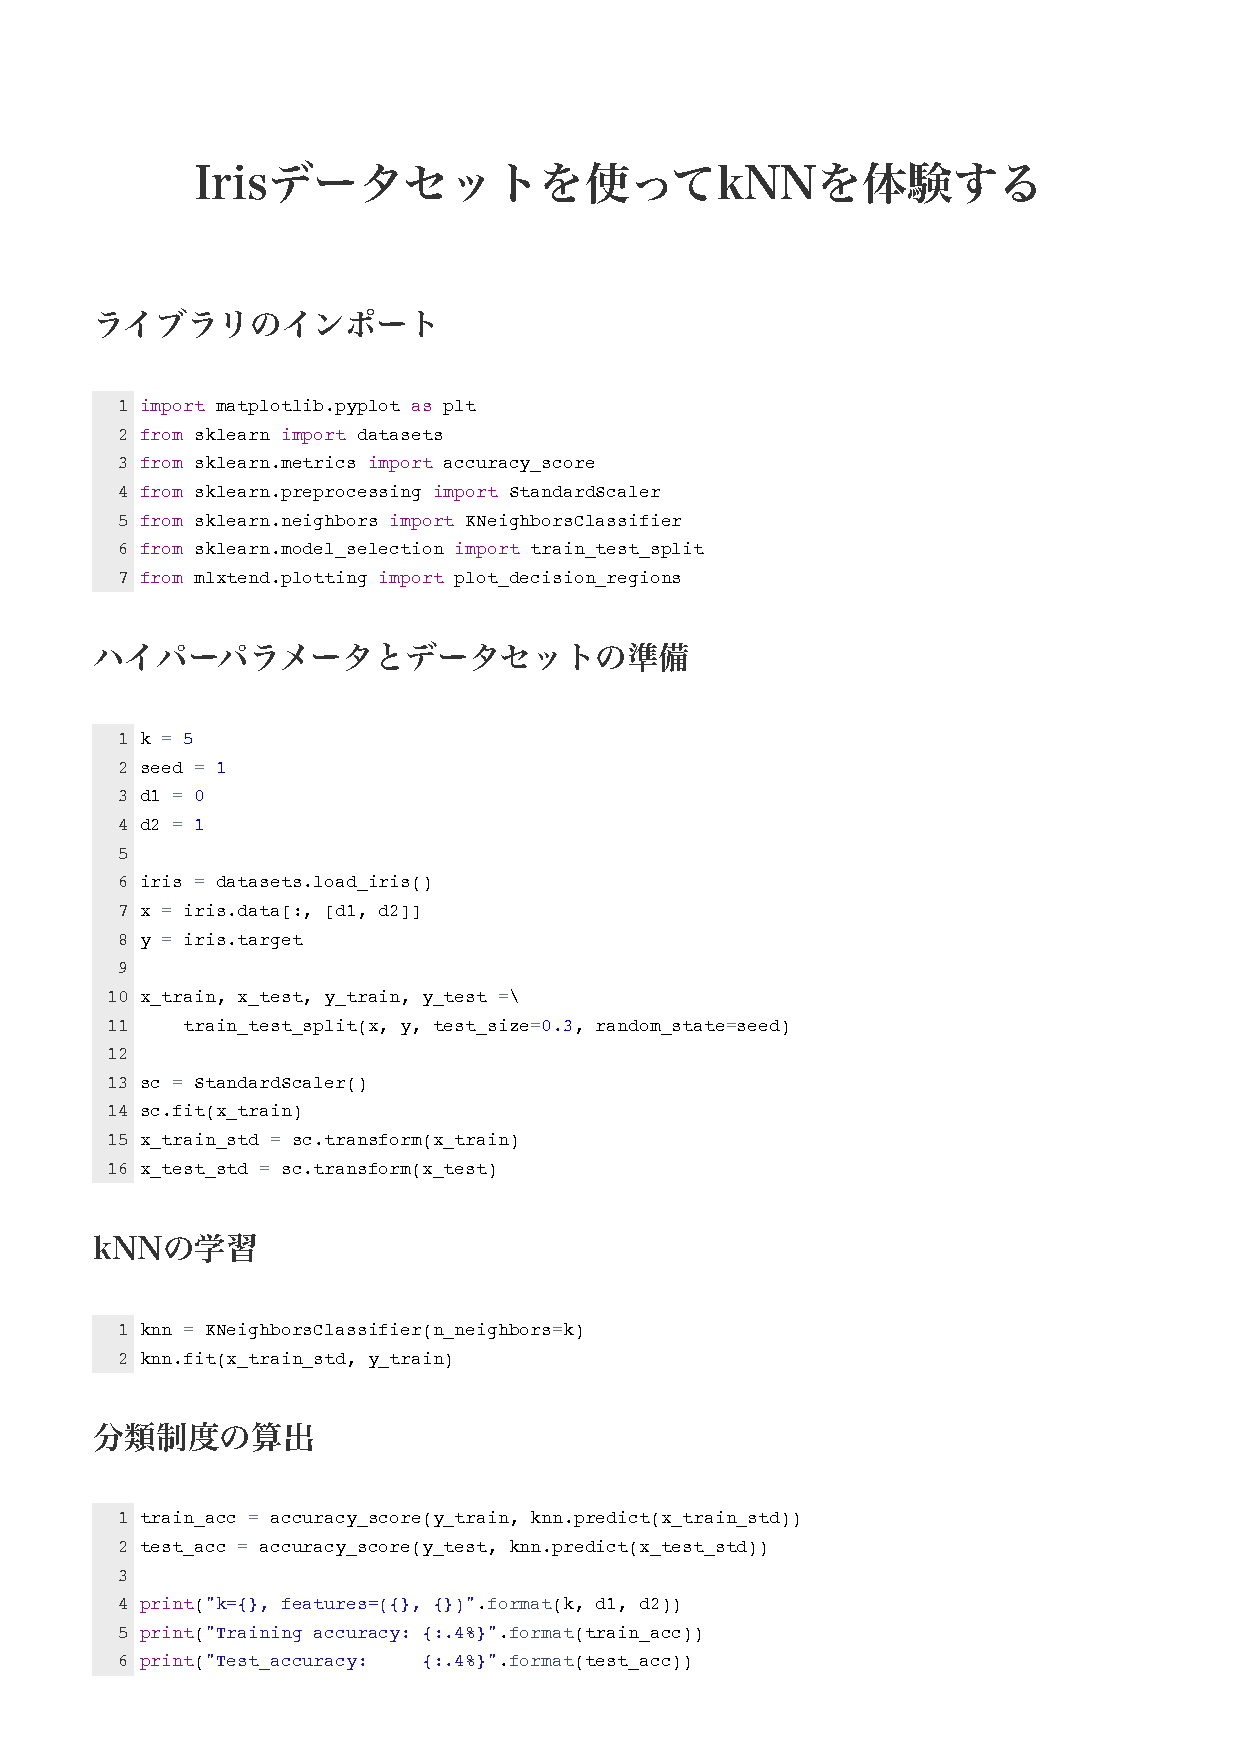
\includepdf[pages=-]{Resources/No1_kNN}

	\chapter{最後に}
	今回は、Pythonの基本的な文法と
	Irisデータセットを使ったkNNによる機械学習を体験しました。
	今後の授業ではPythonといくつかの代表的なライブラリを使って様々な課題
	に挑戦していきます。
	
	また、今回の授業ではPythonの基本的な文法しか触れませんでしたが、
	研究やOSSのコードを読む際に更に複雑な言語の仕様を使う事が多々あります。
	もし興味がある方は、以下の書籍を参照することをお勧めします。
	
	\begin{itemize}
		\item 詳細! Python 3 入門ノート, 大重美幸, ソーテック
		\item 初めてのPython, Mark Lutz, O'REILLY
	\end{itemize}
	
	また、今後の授業でいくつかのアルゴリズムに関して解説を行なっていきますが、
	機械学習分野でさらに詳細な知識を得たい方は、
	以下の入門書をお勧めします。
	
	\begin{itemize}
		\item ゼロから作るDeep Learning, 斎藤康毅, O'REILLY
		\item 機械学習のエッセンス, 加藤公一\footnote{我らがアイドル兵庫県警への抗議として始まった「みんなで逮捕されようプロジェクト」の発起人\url{https://github.com/hamukazu/lets-get-arrested/}} , SBクリエイティブ
	\end{itemize}


	
	\begin{thebibliography}{9}
		\bibitem{python_rl} 久保隆宏, Pythonで学ぶ強化学習 入門から実戦まで, 講談社, 2019
		\bibitem{essence_of_ML} 加藤公一, 機械学習のエッセンス, SBクリエイティブ, 2018
%		\bibitem{comic} 荒木雅弘, マンガでわかる機械学習, オーム社
		\bibitem{python_ML_pro} Sebastian Raschka, Vahid Mirjalili, Python機械学習プログラミング[第2版], 株式会社インプレス, 2018
		\bibitem{TextBook} 福井健一, Pythonと実例で学ぶ機械学習 識別・予測・異常検知, オーム社, 2018
		
	\end{thebibliography}
	
\end{document}
